% 1977 年安徽卷（文科）第 8 题：山顶 D 测山高示意图（按源卷布局）
% DC 垂直于基线 AC（直角在 C，原图未画直角标记），过 D 水平虚线；
% 俯角 30° 弧（水平线到 DA）与 45° 弧（水平线到 DB）标在 D 处，
% 45° 标签按原图写在视线 DA 与 DB 之间。
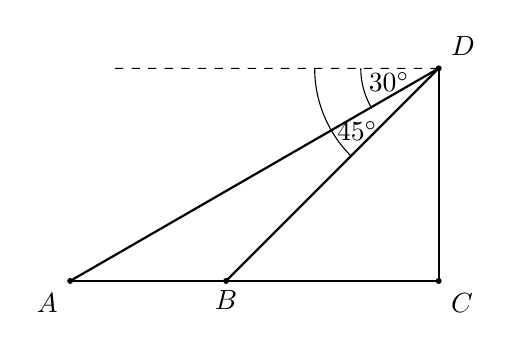
\begin{tikzpicture}[scale=0.9, line join=round]
  \coordinate (A) at (-5.2,0);
  \coordinate (B) at (-3,0);
  \coordinate (C) at (0,0);
  \coordinate (D) at (0,3);
  \draw[thick] (A) -- (C);
  \draw[thick] (C) -- (D);
  \draw[thick] (D) -- (A);
  \draw[thick] (D) -- (B);
  \draw[dashed] (D) -- (-4.6,3);
  \fill (A) circle (1.2pt) node[below left=1pt] {$A$};
  \fill (B) circle (1.2pt) node[below] {$B$};
  \fill (C) circle (1.2pt) node[below right=1pt] {$C$};
  \fill (D) circle (1.2pt) node[above right=1pt] {$D$};
  \draw (-1.1,3) arc[start angle=180, end angle=210, radius=1.1];
  \draw (-1.75,3) arc[start angle=180, end angle=225, radius=1.75];
  \node at (-0.70,2.81) {$30^\circ$};
  \node at (-1.15,2.12) {$45^\circ$};
\end{tikzpicture}
